\section{Ackley Function}
\label{sec:app:test:ackley}

  In the field of optimization, especially within evolutionary algorithms and 
  swarm intelligence, the \emph{Ackley function} serves as a prevalent benchmark 
  function. 
  Named after \textit{David H. Ackley}, who introduced it during his 
  research,\footnote{%
    Ackley, D. H. (1987) \enquote{A connectionist machine for genetic 
    hillclimbing}, Kluwer Academic Publishers, Boston MA.
  } this function is particularly challenging for optimization algorithms due to
  its property of possessing a large number of local minima, despite having a
  single global minimum.
  This trait can often cause such algorithms to become entrapped in local
  minima.

\begin{definition}[Ackley Function]
  The \emph{Ackley Function}, denoted as \(f: \mathbb{R}^2 \rightarrow 
  \mathbb{R}\), is mathematically expressed as:

  \begin{equation}
    \label{eq:app:test:ackley}
    f(x,\, y) = -20\, e^{-0.2 \sqrt{0.5 (x^2 + y^2)}} - 
      e^{0.5\, [\cos(2 \pi x) + \cos(2\pi y)]} + e + 20
  \end{equation}

  This function is evaluated within the range \(x, y \in [-5,\,5]\).
\end{definition}

The global minimum of the Ackley function is located at \(f(0,\, 0) = 0\). 
Visualizations of the Ackley function are depicted as a contour plot and a 
surface plot in \vref{fig:app:test:ackley}.

\begin{figure}[ht!]
  \centering
  \begin{subfigure}[b]{0.45\textwidth}
    \centering
    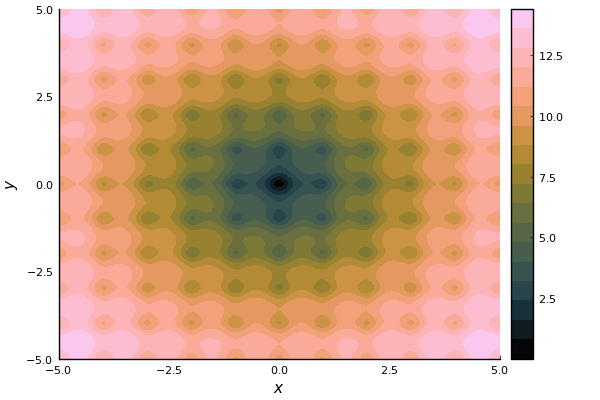
\includegraphics[width=\textwidth]{img/test_functions/ackley_contour.png}
    \caption{Contour plot of the Ackley Function}
  \end{subfigure}
  \hfill
  \begin{subfigure}[b]{0.45\textwidth}
    \centering
    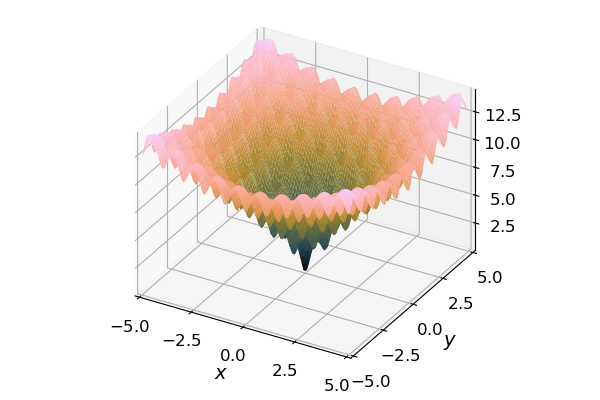
\includegraphics[width=\textwidth]{img/test_functions/ackley_surface.png}
    \caption{Surface plot of the Ackley Function}
  \end{subfigure}
  \caption{
    Illustrations of the Ackley Function with the global minimum indicated by a
    red dot.
  }
  \label{fig:app:test:ackley}
\end{figure}
